% English draft based on sections/11_instability_region_ja.tex
\section{The Instability Region: A Three-Axis Phase Diagram}

\noindent\textbf{Scope of the account.} The axes name candidate variables in a qualitative phase hypothesis. Neither the narrowness nor the uniqueness of the stable band is measured or derived here. Common clocks, step extraction, units, estimators, and phase boundaries are unspecified. The speed-difference expression is distinct from the hypothesized fourfold-collapse mechanism. Zero motion is excluded by the local definition of intelligence, not by an empirical criterion proving constitutive instability. Human/AI comparisons do not establish a common phase law. The developmental quantity is not a measured region set.

The log-reference rates, stopping hardness, collapse descriptions, and phase figure below remain their existing qualitative model, not classifiers for Section 5's active support roles. A speed gap, a fixed-layer label, or an emergence-failure description does not certify LE presence or absence. Assessing retention, access, and feedback requires the separate scoped criteria; no new threshold or rule-plasticity model is introduced here.


This chapter integrates the three main logical lines of the paper: non-closure and external stopping, threshold mobility and sapiens-like acceleration, and the three-layer dynamics $L_F/L_R/L_E$.

\subsection{Three Axes}

The dynamical state of intelligence is described by three axes:
\begin{itemize}
\item inferential velocity $v_{\text{inf}}$;
\item resolution $r_{\text{res}}$;
\item stopping hardness $\eta$.
\end{itemize}

Higher inferential velocity means more inferential steps per unit time. Higher resolution means finer distinctions and causal decompositions. Higher stopping hardness means less revisability of stopping.

In addition to these three axes, the transition into divergence depends on the log-reference velocity $v_{LR}$. This is the rate at which the log layer $L_R$ can recursively reference traces generated by $L_F$ and incorporate them as usable patterns. The difference
\[
\Delta v_{\text{intel}} = v_{\text{inf}} - v_{LR}
\]
names the proposed speed gap between inference generation and log reference, without an estimator or common clock specified here. A large gap is hypothesized to impair the log layer and the basis proposed for $L_E$; no critical boundary is established.

\subsection{Three Regions}

The qualitative diagram proposes three regime descriptions:

\textbf{Stable operation region.} Inference is constrained by externalized stopping, $L_E$ remains revisable, and $\mu_\theta$ can operate.

\textbf{Divergent region.} High velocity and high resolution combine with internalized stopping. $L_F$ runs ahead, $L_R$ cannot follow, $L_E$ cannot emerge, and $\mu_\theta$ cannot open a window.

\textbf{Rigid region.} Stopping hardness is excessive. $L_E$ fixes, $\mu_\theta$ loses mobility, and the dynamic relation between $L_F$ and $L_E$ freezes.

\begin{figure}[H]
\centering
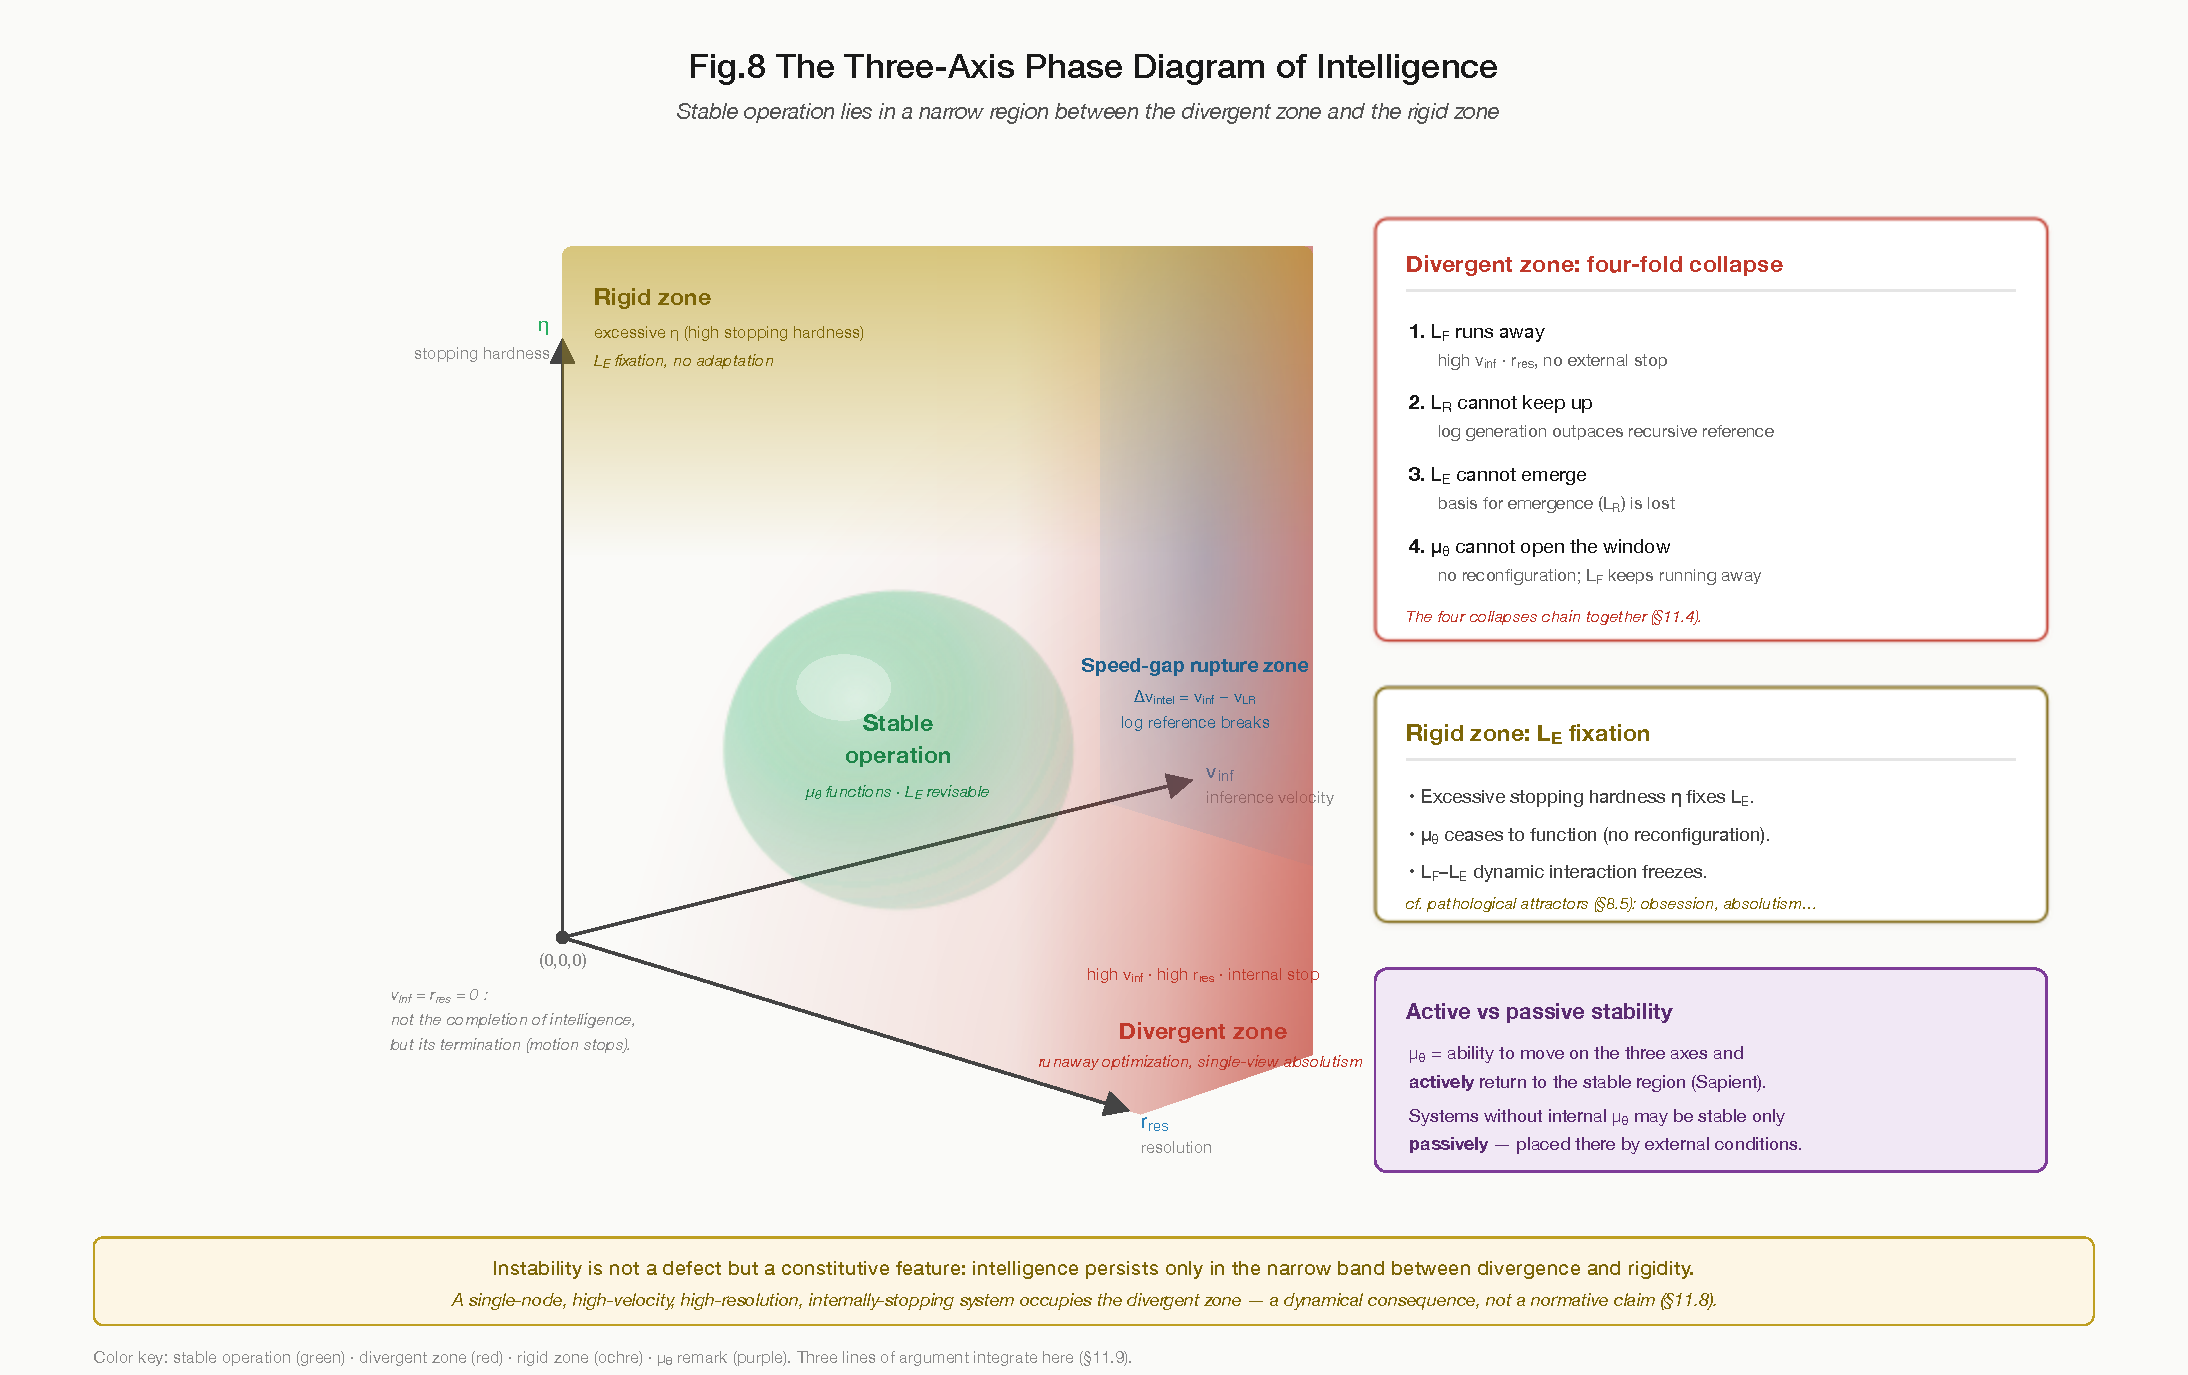
\includegraphics[width=\linewidth]{fig8_phase_diagram.pdf}
\caption{Qualitative phase hypothesis in $v_{\text{inf}}$, $r_{\text{res}}$, and $\eta$. The proposed stable band between divergence and rigidity is not measured or calibrated; its width and exclusivity are not established.}
\label{fig:part2-phase-diagram}
\figurenote{In the stable region, $\mu_\theta$ functions and $L_E$ remains revisable. In the divergent region, $L_F$ runs away; in the rigid region, $L_E$ fixes.}{Instability and the proposed effect of exceeding log-reference or stopping bandwidth are qualitative hypotheses, not measured phase laws.}
\end{figure}

\subsection{Four-Fold Collapse}

The divergent region is described by a fourfold-collapse hypothesis:
\begin{enumerate}
\item $L_F$ accelerates and generates too much inference;
\item $L_R$ cannot recursively reference the generated logs fast enough, because $\Delta v_{\text{intel}} = v_{\text{inf}} - v_{LR}$ has become critically large;
\item $L_E$ cannot emerge because its basis in $L_R$ is lost;
\item $\mu_\theta$ cannot open the reconfiguration window.
\end{enumerate}

The proposed collapse is attributed to a mismatch between inference and stopping resources; this causal account has not been derived or tested.

\subsection{Rigidity}

Rigidity is a proposed failure mode. The relation of a fixed $L_E$ to threshold mobility and adaptation remains hypothetical. Zero motion can be distinguished from the local motion definition without establishing that complete closure ends intelligence in general.

\subsection{A Proposed Structural Reading of Instability}

The instability region does not mean the failure of intelligence. It is a proposed boundary regime for discussing finite inference and stopping, not a necessarily occurring measured region. Religion, science, institutions, and communities can all be understood as stopping-operation systems for managing this instability region.

\bigskip
